\documentclass[10pt,letterpaper]{article}
\usepackage[margin=0.77in,headheight=19pt,headsep=0.26in,footskip=0.38in]{geometry}
\usepackage[T1]{fontenc}
\usepackage[utf8]{inputenc}
\usepackage{lmodern,microtype,tabularx,longtable,array,booktabs,xcolor,colortbl}
\usepackage{enumitem,fancyhdr,lastpage,hyperref,needspace,graphicx}
\usepackage{pdflscape}
\usepackage{tikz}
\usetikzlibrary{arrows.meta,positioning,shapes.geometric}
\definecolor{navy}{HTML}{15334B}
\definecolor{blue}{HTML}{1C6E91}
\definecolor{light}{HTML}{EAF3F7}
\definecolor{rulegrey}{HTML}{D3DEE4}
\definecolor{ink}{HTML}{263748}
\definecolor{muted}{HTML}{596B78}
\hypersetup{colorlinks=true,linkcolor=blue,urlcolor=blue,pdfauthor={CCoE Documentation Suite},pdfsubject={Project management and governance documentation}} 
\setlength\parindent{0pt}
\setlength\parskip{5pt}
\setlist[itemize]{leftmargin=*,itemsep=2pt,topsep=2pt}
\setlist[enumerate]{leftmargin=*,itemsep=4pt,topsep=2pt}
\renewcommand\arraystretch{1.25}
\pagestyle{fancy}
\fancyhf{}
\fancyhead[L]{\footnotesize\sffamily\color{muted} CLOUD CENTER OF EXCELLENCE}
\fancyhead[R]{\footnotesize\sffamily\color{muted} \DocId\quad|\quad\DocPhase}
\fancyfoot[L]{\scriptsize\color{muted} Internal working template \textbar{} Version 1.0}
\fancyfoot[R]{\scriptsize\color{muted} \thepage\ of \pageref{LastPage}}
\renewcommand\headrulewidth{0.35pt}
\newcommand{\topruleline}{\color{blue}\rule{\linewidth}{1.2pt}\color{black}\par}
\newcommand{\fieldline}[1]{\noindent\textbf{#1}\hspace{.5em}\rule{.62\linewidth}{.45pt}\par\vspace{4pt}}
\newcommand{\writelines}{\par\noindent\color{rulegrey}\rule{\linewidth}{.35pt}\par\vspace{7pt}\rule{\linewidth}{.35pt}\color{black}\par\vspace{7pt}}
\newcommand{\docsection}[1]{\par\Needspace{5\baselineskip}\vspace{8pt}{\large\sffamily\bfseries\color{navy}#1}\par\vspace{2pt}{\color{rulegrey}\rule{\linewidth}{.6pt}}\par}
\newcommand{\smallsection}[1]{\par\Needspace{3\baselineskip}\vspace{5pt}{\normalsize\sffamily\bfseries\color{blue}#1}\par}

\newcommand{\DocId}{1.3}
\newcommand{\DocPhase}{Initiating}
\begin{document}
{\color{navy}\sffamily\Huge\bfseries Stakeholder Analysis Matrix}\par
{\color{blue}\sffamily\large Document 1.3 \textbar{} Initiating Process Group}\par\vspace{5pt}\topruleline
\vspace{7pt}
\begin{tabularx}{\linewidth}{@{}p{1.16in}X p{1.02in}X@{}}\textbf{Project} & \rule{\linewidth}{.4pt} & \textbf{Prepared} & \rule{\linewidth}{.4pt}\\[6pt]\textbf{Owner} & \rule{\linewidth}{.4pt} & \textbf{Version} & 1.0 / \rule{.75in}{.4pt}\\[6pt]\textbf{Approver} & \rule{\linewidth}{.4pt} & \textbf{Status} & Draft / Reviewed / Approved\\\end{tabularx}
\docsection{01 \quad Proposed implementation guidance}
\textit{This section is implementation guidance added by the suite. It is not pre-populated source project data.}\par\vspace{2pt}\noindent
\begin{tabularx}{\linewidth}{@{}p{1.3in}X@{}}
\textbf{Suggested owner} & Stakeholder Engagement Lead\\
\textbf{Control objective} & Approve initiation authority and stakeholders before detailed baselining.\\
\textbf{Related artifacts} & 1.2 Stakeholder Register; 2.38 Stakeholder Management Plan\\
\textbf{Evidence to retain} & Completed and approved form; linked decisions, baselines, work items, and sign-offs as applicable.\\
\end{tabularx}
\docsection{02 \quad Source-derived working form}
\textit{Source labels, checklist wording, and tabular structure are retained from the uploaded 1.3 Stakeholder Analysis Matrix.docx. Blank entry cells are intended for completion. Where a source example is not project data, it remains explicitly identified as an example.}\par
\begin{center}
\begingroup
\setlength\tabcolsep{2.0pt}
\footnotesize
\renewcommand\arraystretch{1.55}
\begin{longtable}{|>{\raggedright\arraybackslash}p{3.245in}|>{\raggedright\arraybackslash}p{3.245in}|}
\hline
\rowcolor{light}
\rule{0pt}{11pt}\hspace{0pt} & \rule{0pt}{11pt}\hspace{0pt} \\ \hline
\endfirsthead
\hline\rowcolor{light} \rule{0pt}{11pt}\hspace{0pt} & \rule{0pt}{11pt}\hspace{0pt} \\ \hline
\endhead
\rule{0pt}{11pt}\hspace{0pt} & \rule{0pt}{11pt}\hspace{0pt} \\ \hline
\rule{0pt}{11pt}\hspace{0pt} & \rule{0pt}{11pt}\hspace{0pt} \\ \hline
\rule{0pt}{11pt}\hspace{0pt} & \rule{0pt}{11pt}\hspace{0pt} \\ \hline
\rule{0pt}{11pt}\hspace{0pt} & \rule{0pt}{11pt}\hspace{0pt} \\ \hline
\end{longtable}
\endgroup
\end{center}

\smallsection{Interest}
\writelines
\smallsection{Stakeholder power--interest map (working grid)}
\begin{center}
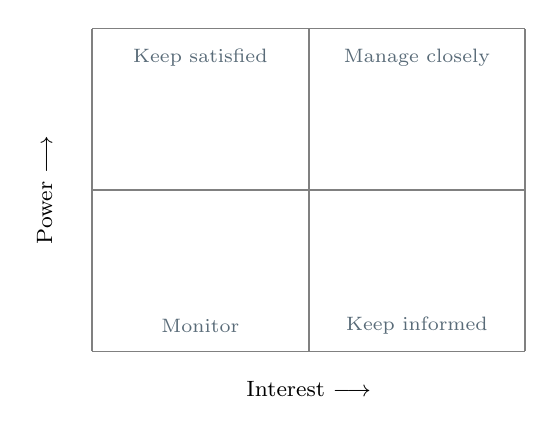
\begin{tikzpicture}[x=2.75cm,y=2.05cm]
\draw[step=1,black!50,line width=.65pt] (0,0) grid (2,2);
\node[align=center,font=\scriptsize,text=muted] at (.5,1.82){Keep satisfied};
\node[align=center,font=\scriptsize,text=muted] at (1.5,1.82){Manage closely};
\node[align=center,font=\scriptsize,text=muted] at (.5,.16){Monitor};
\node[align=center,font=\scriptsize,text=muted] at (1.5,.16){Keep informed};
\node[rotate=90,font=\footnotesize] at (-.22,1){Power $\longrightarrow$};
\node[font=\footnotesize] at (1,-.23){Interest $\longrightarrow$};
\end{tikzpicture}
\end{center}
\textit{Proposed annotations: quadrant engagement labels are guidance added for practical use; plot identified stakeholders here.}
\docsection{03 \quad Source diagnostic checklist}
\textit{The following questions are preserved as diagnostic prompts from the original file, including any broad or sector-specific wording. They do not indicate that a condition has been verified. Mark N/A where not applicable.}
\begingroup\small\begin{enumerate}[leftmargin=2.1em, itemsep=4pt]
\item[1.] Guiding question: who shall you involve in the making of the stakeholder map?
\item[2.] Environmental effects?
\item[3.] Reliability of data, plan predictability?
\item[4.] Identify the stakeholders levels most frequently used -or at least sought- in your Cloud Center of Excellence projects and for which purpose?
\item[5.] Why do you need to manage Cloud Center of Excellence project Risk?
\item[6.] Innovative aspects?
\item[7.] What tools would help you communicate?
\item[8.] Price, value, quality?
\item[9.] Gaps in capabilities?
\item[10.] Competitor intentions - various?
\item[11.] How affected by the problem(s)?
\item[12.] Is there a reason why you are or are not not using an external rating system?
\item[13.] What resources might the stakeholder bring to the Cloud Center of Excellence project?
\item[14.] Guiding question: what is the issue at stake?
\item[15.] Processes, systems, it, communications?
\item[16.] Seasonality, weather effects?
\item[17.] Insurmountable weaknesses?
\item[18.] Financial reserves, likely returns?
\item[19.] What coalitions might build around the issues being tackled?
\item[20.] Information and research?
\item[21.] Management cover, succession?
\item[22.] Who is most interested in information about the topic and/or has previously initiated interest?
\item[23.] Market developments?
\item[24.] Who can contribute financial or technical resources towards the work?
\item[25.] What is the stakeholders name, what is function?
\end{enumerate}\endgroup
\docsection{04 \quad Review and approval record}
\begin{tabularx}{\linewidth}{|p{1.1in}|X|p{1.05in}|p{1.1in}|}\hline\rowcolor{light}\textbf{Stage} & \textbf{Reviewer / role} & \textbf{Date} & \textbf{Disposition}\\\hline Draft review & & & \\ \hline Technical / control & & & \\ \hline Approval & & & \\ \hline\end{tabularx}
\vspace{5pt}\textit{Documented decisions, deviations, and required follow-up:}\writelines
\end{document}
